\documentclass[aspectratio=169, table, 12pt]{beamer}

\usepackage{colortbl}
\usepackage{xcolor}
\usepackage{listings}
\usepackage{tabularx}
\usepackage{tikz}
\usetikzlibrary{arrows.meta, positioning, calc, fit, shapes.geometric}

\makeatletter
\def\input@path{{../theme/}}
\makeatother
\graphicspath{{../theme/}{../../figures/}}
\usetheme{Pradita}

\definecolor{praditagreen}{RGB}{37, 113, 71}

% Tema membuat garis tabel berwarna putih. Dikembalikan agar tabel terbaca.
\arrayrulecolor{black}
\setlength{\arrayrulewidth}{0.5pt}

% Kolom X rata kiri, dipakai pada tabel dengan kolom X yang sempit, agar
% spasi antarkata tidak meregang.
\newcolumntype{Y}{>{\raggedright\arraybackslash}X}

\lstdefinelanguage{bash}{
  keywords={},
  basicstyle=\ttfamily\scriptsize,
  ndkeywords={cd, coverage, curl, diff, docker, echo, npm, npx, python,
              python3, pytest, source},
  ndkeywordstyle=\color{purple}\bfseries,
  sensitive=true,
  commentstyle=\color{gray},
  numbers=none,
  breaklines=true,
  frame=lines,
  backgroundcolor=\color{lightgray!10},
  tabsize=2,
  comment=[l]{\#},
  showstringspaces=false
}

\lstdefinelanguage{TypeScript}{
  keywords={const, let, function, return, async, await, try, catch, throw,
            new, if, interface, void, export, import, from, type},
  ndkeywords={Promise, number, string, boolean, test, expect, Page, await},
  basicstyle=\ttfamily\scriptsize,
  keywordstyle=\color{blue}\bfseries,
  ndkeywordstyle=\color{purple}\bfseries,
  sensitive=true,
  commentstyle=\color{gray}\itshape,
  stringstyle=\color{red},
  numbers=none,
  breaklines=true,
  frame=lines,
  backgroundcolor=\color{lightgray!10},
  tabsize=2,
  comment=[l]{//},
  morestring=[b]",
  showstringspaces=false
}

% Gaya Python disamakan dengan naskah bab, tanpa nomor baris.
\lstdefinestyle{PythonStyle}{
  language=Python,
  basicstyle=\ttfamily\scriptsize,
  morekeywords={with, as, yield, async, await, match, case},
  keywordstyle=\color{blue}\bfseries,
  emph={pytest, psycopg, Mock, given, strategies},
  emphstyle=\color{purple}\bfseries,
  commentstyle=\color{gray}\itshape,
  stringstyle=\color{red},
  numbers=none,
  breaklines=true,
  frame=lines,
  backgroundcolor=\color{lightgray!10},
  tabsize=2,
  showstringspaces=false
}

% File mutu dan kontrak ditampilkan apa adanya, sehingga butuh gaya JSON.
\lstdefinelanguage{json}{
  basicstyle=\ttfamily\scriptsize,
  stringstyle=\color{red},
  commentstyle=\color{gray},
  numbers=none,
  breaklines=true,
  frame=lines,
  backgroundcolor=\color{lightgray!10},
  tabsize=2,
  showstringspaces=false,
  morestring=[b]"
}


% Contoh pipeline ditampilkan apa adanya, sehingga butuh gaya YAML sendiri.
\lstdefinelanguage{yaml}{
  basicstyle=\ttfamily\scriptsize,
  keywordstyle=\color{blue}\bfseries,
  commentstyle=\color{gray}\itshape,
  stringstyle=\color{red},
  showstringspaces=false,
  breaklines=true,
  frame=lines,
  numbers=none,
  backgroundcolor=\color{lightgray!10},
  tabsize=2,
  morecomment=[l]{\#},
  literate=
    *{-}{{{\color{blue}\bfseries-}}}1
     {:}{{{\color{blue}\bfseries:}}}1
}

\title{\Huge Cloud Deployment,\\ \vspace{10pt} DevOps, dan Observability}
\subtitle{IF140303 - Pengembangan Aplikasi Web}
\author{\textbf{Alfa Yohannis}}

\begin{document}

\frame{\titlepage}

\begin{frame}[fragile]
  \frametitle{Isi Pertemuan}
  \vspace{14pt}
  \begin{columns}[t]
    \column{0.5\textwidth}
    {\small\tableofcontents[sections={1-7}]}

    \column{0.5\textwidth}
    {\small\tableofcontents[sections={8-14}]}
  \end{columns}
\end{frame}

\begin{frame}{\hfill}
  \centering
  \Huge{\textbf{Apa yang berubah ketika\\aplikasi dijalankan di tempat lain?}}
\end{frame}

\section{Tujuan dan Kerangka Bahasan}

\begin{frame}{\hfill}
  \centering
  \Huge{\textbf{Tujuan dan Kerangka Bahasan}}
\end{frame}

\begin{frame}{{\Large Tujuan Pembelajaran}}
  \vspace{10pt}
  \begin{itemize}
    \item Mengemas satu layanan sebagai \textit{container} yang setelannya
          datang dari \textit{environment}, lalu menjalankan dua versi dari
          artefak yang sama persis.
    \item Menjalankan rilis \textit{blue-green}, \textit{canary}, dan
          \textit{rollback} lewat satu \textit{reverse proxy}, lalu mengukur
          pembagian permintaan yang benar-benar terjadi.
    \item Menginstrumentasi layanan dengan \textit{log}, metrik, dan
          \textit{trace}, lalu menilainya terhadap SLO sebagai alarm yang
          keluar dengan status gagal.
  \end{itemize}
\end{frame}

\begin{frame}{{\Large Tiga Pertanyaan Praktis}}
  \vspace{12pt}
  \begin{itemize}
    \item Bagaimana satu artefak yang sama dijalankan di lingkungan berbeda
          tanpa diubah isinya?
    \item Bagaimana versi baru dinaikkan tanpa membuat seluruh pengunjung
          menanggung risikonya?
    \item Bagaimana keadaan sistem diketahui dari luar, tanpa menebak dari
          keluhan pengguna?
  \end{itemize}
  \vspace{8pt}
  {\small Demonya kecil: dua versi layanan di belakang satu \textit{reverse
  proxy}, seluruhnya dengan Python pustaka standar, ditambah satu
  \textit{image} berisi satu file.}
\end{frame}

\section{Container dan Twelve-Factor}

\begin{frame}{\hfill}
  \centering
  \Huge{\textbf{Container dan\\Twelve-Factor App}}
\end{frame}

\begin{frame}{{\Large Lima Aturan yang Paling Terasa}}
  \vspace{6pt}
  \centering
  {\footnotesize
  \begin{tabularx}{\textwidth}{lY}
    \hline
    \textbf{Aturan} & \textbf{Wujudnya di demo ini} \\
    \hline
    Setelan dari \textit{environment} & \texttt{VERSI}, \texttt{PORT}, dan \texttt{HOST} dibaca saat proses mulai \\
    \hline
    Satu artefak, banyak lingkungan & Dua versi dari \textit{image} yang sama, beda hanya \textit{environment} \\
    \hline
    Proses tanpa ingatan tetap & Metrik hilang saat proses diganti \\
    \hline
    \textit{Port binding} & Layanan mengikat portnya sendiri \\
    \hline
    \textit{Log} sebagai aliran peristiwa & Satu baris JSON per permintaan ke stdout \\
    \hline
  \end{tabularx}}
\end{frame}

\begin{frame}{{\Large Satu Pelanggaran Kecil, Akibat Besar}}
  \vspace{12pt}
  \begin{itemize}
    \item Layanan semula mengikat ke \texttt{127.0.0.1}, dan itu bekerja
          dengan baik di komputer sendiri.
    \item Di dalam \textit{container}, alamat itu berarti container itu
          sendiri, sehingga port yang dipublikasikan tidak pernah terjawab.
    \item Perbaikannya satu baris: alamat ikat ikut dibaca dari
          \textit{environment}, dan \textit{image} menyetelnya
          \texttt{0.0.0.0}.
  \end{itemize}
  \vspace{8pt}
  {\small Inilah akibat nyata aturan pertama \textit{twelve-factor}, dan
  cacat semacam ini hanya ketahuan setelah dijalankan.}
\end{frame}

\begin{frame}{{\Large Angka Image dan Containernya}}
  \vspace{6pt}
  \centering
  {\footnotesize
  \begin{tabularx}{\textwidth}{Yr}
    \hline
    \textbf{Ukuran} & \textbf{Hasil} \\
    \hline
    Ukuran \textit{image} & 119 MB \\
    \hline
    Lama \textit{build} pertama, termasuk mengunduh \textit{base image} & 129,7 s \\
    \hline
    Lama \textit{build} ulang, seluruh \textit{layer} tersimpan & 9,5 s \\
    \hline
    Lama sampai siap melayani sesudah \texttt{docker run} & 0,5 s \\
    \hline
  \end{tabularx}}

  \vspace{8pt}
  {\small Selisih 129,7 detik dengan 9,5 detik berasal dari urutan di dalam
  \texttt{Dockerfile}: yang jarang berubah ditulis lebih dahulu.}
\end{frame}

\section{Konfigurasi dan Secret}

\begin{frame}{\hfill}
  \centering
  \Huge{\textbf{Konfigurasi\\dan Manajemen Secret}}
\end{frame}

\begin{frame}{{\Large Tiga Jenis Nilai dari Luar Kode}}
  \vspace{6pt}
  \centering
  {\footnotesize
  \begin{tabularx}{\textwidth}{lYl}
    \hline
    \textbf{Jenis} & \textbf{Contoh di Bab 9} & \textbf{Berubahnya} \\
    \hline
    Setelan proses & \texttt{VERSI}, \texttt{PORT}, \texttt{HOST} & Saat proses mulai \\
    \hline
    Setelan operasional & Bobot rilis di \texttt{rilis.json} & Kapan saja, tanpa menyalakan ulang \\
    \hline
    \textit{Secret} & Kunci sesi, kata sandi basis data & Lewat \textit{environment} saja \\
    \hline
  \end{tabularx}}

  \vspace{8pt}
  {\small Baris tengah yang membuat rilis pada pertemuan ini mungkin: proxy
  membaca bobotnya pada tiap permintaan.}
\end{frame}

\section{CI/CD dan Infrastructure as Code}

\begin{frame}{\hfill}
  \centering
  \Huge{\textbf{CI/CD dan\\Infrastructure as Code}}
\end{frame}

\begin{frame}[fragile]{{\Large Urutan Tahap Pipeline}}
  \vspace{2pt}
\begin{lstlisting}[language=yaml]
      - name: Analisis statis
        run: ruff check sources/chapter09

      - name: Uji unit dan integrasi
        run: pytest -q sources/chapter06

      - name: Bangun image
        run: docker build -t awe9-layanan sources/chapter09
\end{lstlisting}
  \vspace{4pt}
  {\small Urutannya sama seperti Bab 6: yang paling murah dan paling sering
  gagal dijalankan lebih dahulu. IaC membawa gagasan yang sama ke
  infrastrukturnya, dan \texttt{docker-compose.yml} adalah bentuk paling
  sederhananya.}
\end{frame}

\section{Reverse Proxy}

\begin{frame}{\hfill}
  \centering
  \Huge{\textbf{Reverse Proxy,\\Cloud, dan Edge}}
\end{frame}

\begin{frame}{{\Large Satu Tempat untuk Semua Keputusan}}
  \vspace{10pt}
  \centering
  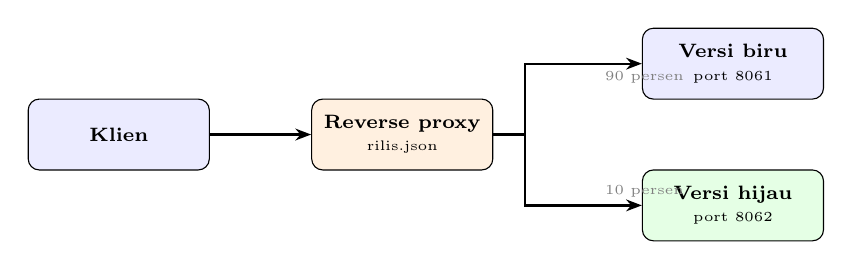
\begin{tikzpicture}[
    font=\scriptsize,
    kotak/.style={draw, rounded corners, minimum height=0.9cm,
                  minimum width=2.3cm, align=center, font=\scriptsize\bfseries},
    panah/.style={-{Stealth[length=2mm]}, thick}
  ]
    \node[kotak, fill=blue!8] (klien) at (0,0) {Klien};
    \node[kotak, fill=orange!12] (proxy) at (3.6,0) {Reverse proxy\\{\tiny\mdseries rilis.json}};
    \node[kotak, fill=blue!8] (biru) at (7.8,0.9) {Versi biru\\{\tiny\mdseries port 8061}};
    \node[kotak, fill=green!10] (hijau) at (7.8,-0.9) {Versi hijau\\{\tiny\mdseries port 8062}};

    \draw[panah] (klien) -- (proxy);
    \draw[panah] (proxy.east) -- ++(0.4,0) |- (biru.west);
    \draw[panah] (proxy.east) -- ++(0.4,0) |- (hijau.west);
    \node[font=\tiny, gray, anchor=east] at (7.3,0.72) {90 persen};
    \node[font=\tiny, gray, anchor=east] at (7.3,-0.72) {10 persen};
  \end{tikzpicture}

  \vspace{10pt}
  {\small Di \textit{cloud} peran itu dipegang \textit{load balancer}
  penyedia, di \textit{edge} dipegang jaringan titik terdekat. Bentuknya
  berbeda, keputusannya sama.}
\end{frame}

\section{Blue-Green, Canary, dan Rollback}

\begin{frame}{\hfill}
  \centering
  \Huge{\textbf{Blue-Green, Canary,\\dan Rollback}}
\end{frame}

\begin{frame}[fragile]{{\Large Seluruh Mekanismenya, Empat Baris}}
  \vspace{2pt}
\begin{lstlisting}[style=PythonStyle]
def pilih_tujuan(rilis, nomor_permintaan):
  """Memilih versi tujuan menurut bobot pada file rilis.

  Pemilihannya berurutan, bukan acak, supaya hasilnya dapat diulang: dari
  tiap seratus permintaan, tepat sebanyak bobot yang menuju versi kedua.
  """
  bobot_kedua = rilis["bobot_persen_kedua"]
  if nomor_permintaan % 100 < bobot_kedua:
    return rilis["versi_kedua"]
  return rilis["versi_pertama"]
\end{lstlisting}
\end{frame}

\begin{frame}{{\Large Tiga Tahap Rilis, Diukur}}
  \vspace{6pt}
  \centering
  {\footnotesize
  \begin{tabularx}{\textwidth}{Yrrrr}
    \hline
    \textbf{Tahap} & \textbf{Minta} & \textbf{Biru} & \textbf{Hijau} & \textbf{Gagal} \\
    \hline
    \textit{Canary} 10 persen & 500 & 450 & 50 & 2 \\
    \hline
    \textit{Blue-green}, seluruhnya hijau & 100 & 0 & 100 & 4 \\
    \hline
    \textit{Rollback}, kembali ke biru & 100 & 100 & 0 & 0 \\
    \hline
  \end{tabularx}}

  \vspace{8pt}
  {\small Versi hijau sengaja dibuat cacat: empat kali lebih lama, dan satu
  dari dua puluh lima permintaannya dijawab 500. Pada \textit{canary} cacat
  itu hanya mengenai 50 dari 500 permintaan.}
\end{frame}

\section{Log, Metrik, dan Trace}

\begin{frame}{\hfill}
  \centering
  \Huge{\textbf{Log, Metrik, dan Trace}}
\end{frame}

\begin{frame}{{\Large Tiga Pertanyaan yang Berbeda}}
  \vspace{6pt}
  \centering
  {\footnotesize
  \begin{tabularx}{\textwidth}{lYl}
    \hline
    \textbf{Keluaran} & \textbf{Wujudnya} & \textbf{Menjawab} \\
    \hline
    \textit{Log} & Satu baris JSON per permintaan ke stdout & Apa yang terjadi \\
    \hline
    Metrik & Teks format Prometheus di \texttt{/metrics} & Bagaimana keadaannya \\
    \hline
    \textit{Trace} & \textit{Trace id} di header \texttt{traceparent} & Ke mana perginya \\
    \hline
  \end{tabularx}}

  \vspace{8pt}
  {\small Sebaran waktu disimpan sebagai histogram: hemat, tetapi persentilnya
  selalu jatuh pada salah satu batas ember.}
\end{frame}

\begin{frame}{{\Large Papan Operasional Sesudah 500 Permintaan}}
  \vspace{6pt}
  \centering
  {\footnotesize
  \begin{tabularx}{\textwidth}{Yrrrrr}
    \hline
    \textbf{Versi} & \textbf{Minta} & \textbf{Gagal} & \textbf{\% gagal} & \textbf{Rata ms} & \textbf{p95 ms} \\
    \hline
    biru & 450 & 0 & 0,0 & 5,1 & 10 \\
    \hline
    hijau & 50 & 2 & 4,0 & 20,1 & 25 \\
    \hline
  \end{tabularx}}

  \vspace{8pt}
  {\small Perbedaan kedua versi terbaca dari metrik, tanpa perlu membaca
  kodenya.}
\end{frame}

\begin{frame}[fragile]{{\Large Menelusuri Satu Permintaan}}
  \vspace{2pt}
\begin{lstlisting}[language=bash]
grep -h "300a032b60413b55e53009cc0660f240" proxy.log hijau.log

# Keluarannya, dirapikan:
#   hijau    /api/katalog   status 500   20.2 ms
#   proxy    /api/katalog   status 500   22.2 ms
\end{lstlisting}
  \vspace{4pt}
  {\small Dua baris itu menjawab yang tidak dapat dijawab metrik maupun
  \textit{log} sendirian: kegagalannya berasal dari layanan hijau, dan
  selisih 2 milidetik adalah biaya penerusan proxy.}
\end{frame}

\section{SLI dan SLO}

\begin{frame}{\hfill}
  \centering
  \Huge{\textbf{Dasar SLI dan SLO}}
\end{frame}

\begin{frame}{{\Large Batas yang Disepakati Lebih Dahulu}}
  \vspace{12pt}
  \begin{itemize}
    \item \textbf{SLI} adalah angka yang mewakili pengalaman pengguna,
          misalnya persentase permintaan yang berhasil.
    \item \textbf{SLO} adalah batas yang disepakati untuk angka itu,
          misalnya 99 persen.
    \item Selisih 100 persen dengan SLO adalah \textit{error budget}: dengan
          SLO 99 persen, dari 500 permintaan ada jatah 5 yang boleh gagal.
  \end{itemize}
  \vspace{8pt}
  {\small Jatah itulah yang membuat rilis mungkin: selama budgetnya belum
  habis, versi baru boleh dinaikkan.}
\end{frame}

\begin{frame}{{\Large Penilaian Alarm}}
  \vspace{6pt}
  \centering
  {\footnotesize
  \begin{tabularx}{\textwidth}{Yrrl}
    \hline
    \textbf{Tujuan} & \textbf{SLO} & \textbf{Terukur} & \textbf{Verdict} \\
    \hline
    biru: ketersediaan persen & 99,0 & 100,0 & lolos \\
    \hline
    biru: p95 milidetik & 50 & 10 & lolos \\
    \hline
    hijau: ketersediaan persen & 99,0 & 96,0 & LANGGAR \\
    \hline
    hijau: p95 milidetik & 50 & 25 & lolos \\
    \hline
  \end{tabularx}}

  \vspace{6pt}
  {\footnotesize Alarm keluar dengan status 1, sama seperti gerbang Bab 5
  sampai 7. Perhatikan baris terakhir: versi hijau dua setengah kali lebih
  lambat, tetapi masih di bawah batas. Pelan belum tentu melanggar.}
\end{frame}

\section{Persiapan Latihan}

\begin{frame}{\hfill}
  \centering
  \Huge{\textbf{Persiapan Latihan}}
\end{frame}

\begin{frame}[fragile]{{\Large Tiga Proses, Satu Perintah Masing-Masing}}
  \vspace{2pt}
\begin{lstlisting}[language=bash]
cd sources/chapter09
VERSI=biru PORT=8061 python3 aplikasi.py > biru.log &
VERSI=hijau PORT=8062 python3 aplikasi.py > hijau.log &
python3 proxy.py > proxy.log &
\end{lstlisting}
  \vspace{4pt}
  {\small Docker hanya dipakai pada latihan terakhir. Seluruh pengukuran
  diarahkan ke layanan di komputer sendiri, dengan beban setara satu
  pengguna.}
\end{frame}

\section{Latihan 1: Rilis Canary}

\begin{frame}{\hfill}
  \centering
  \Huge{\textbf{Latihan 1\\Menjalankan Rilis Canary}}
\end{frame}

\begin{frame}[fragile]{{\Large Langkah Kerja dan Perintahnya}}
  \vspace{2pt}
  {\footnotesize Pastikan bobotnya 10, kirim 200 permintaan, lalu ubah
  menjadi 50 dan kirim lagi. Proxy tidak perlu dinyalakan ulang.}
  \vspace{2pt}
\begin{lstlisting}[language=bash]
python3 ukur-rilis.py 200

# Keluarannya:
# Permintaan   : 200
#   biru     :  180 permintaan (90.0%)
#   hijau    :   20 permintaan (10.0%)
#   status 200 :  200 permintaan
# p50          : 6.7 ms
# p95          : 21.9 ms
\end{lstlisting}
\end{frame}

\begin{frame}{{\Large Lembar Isian Latihan 1}}
  \vspace{6pt}
  \centering
  {\footnotesize
  \begin{tabularx}{\textwidth}{Yrrrr}
    \hline
    \textbf{Bobot hijau} & \textbf{Minta} & \textbf{Biru} & \textbf{Hijau} & \textbf{Gagal} \\
    \hline
    10 persen & \dots & \dots & \dots & \dots \\
    \hline
    50 persen & \dots & \dots & \dots & \dots \\
    \hline
    100 persen & \dots & \dots & \dots & \dots \\
    \hline
    0 persen, sesudah \textit{rollback} & \dots & \dots & \dots & \dots \\
    \hline
  \end{tabularx}}

  \vspace{6pt}
  {\footnotesize Pertanyaan: berapa permintaan yang menanggung risiko pada
  tiap bobot, mengapa pembagiannya tepat dan tidak meleset, dan apa
  pertimbangan memilih bobot pertama sebuah rilis?}
\end{frame}

\section{Latihan 2: Papan Operasional}

\begin{frame}{\hfill}
  \centering
  \Huge{\textbf{Latihan 2\\Membaca Papan Operasional}}
\end{frame}

\begin{frame}[fragile]{{\Large Dari Metrik Mentah ke Papan}}
  \vspace{2pt}
\begin{lstlisting}[language=bash]
curl -s http://127.0.0.1:8061/metrics | head -8
python3 papan.py

# Keluarannya:
#   Versi                       Minta   Gagal  % gagal   Rata ms   p95 ms
#   biru                          450       0      0.0       5.1       10
#   hijau                          50       2      4.0      20.1       25
\end{lstlisting}
  \vspace{4pt}
  {\footnotesize Pertanyaan: mengapa p95 selalu jatuh pada angka yang sama
  seperti 10 atau 25, dan apa yang hilang bila sebaran waktu disimpan sebagai
  rata-rata saja?}
\end{frame}

\section{Latihan 3: Menelusuri Permintaan}

\begin{frame}{\hfill}
  \centering
  \Huge{\textbf{Latihan 3\\Menelusuri Satu Permintaan}}
\end{frame}

\begin{frame}[fragile]{{\Large Mengambil Trace Id lalu Mencarinya}}
  \vspace{2pt}
\begin{lstlisting}[language=bash]
curl -sI http://127.0.0.1:8060/api/katalog | grep -i x-trace-id
grep -h "300a032b60413b55e53009cc0660f240" proxy.log hijau.log

# Keluarannya, dirapikan:
#   hijau    /api/katalog   status 500   20.2 ms
#   proxy    /api/katalog   status 500   22.2 ms
\end{lstlisting}
  \vspace{4pt}
  {\footnotesize Pertanyaan: berapa biaya penerusan proxy dan dari angka mana
  Anda mengetahuinya, serta apa yang terjadi bila proxy tidak meneruskan
  header \texttt{traceparent}?}
\end{frame}

\section{Latihan 4: SLO dan Container}

\begin{frame}{\hfill}
  \centering
  \Huge{\textbf{Latihan 4\\SLO dan Container}}
\end{frame}

\begin{frame}[fragile]{{\Large Alarm lalu Container}}
  \vspace{2pt}
\begin{lstlisting}[language=bash]
python3 alarm.py
echo $?
docker build -t awe9-layanan .
docker run -d --name awe9-uji -e VERSI=biru -p 8065:8061 awe9-layanan
curl -s http://127.0.0.1:8065/sehat

# Keluarannya:
# Gagal: 1 tujuan SLO tidak terpenuhi.
# 1
# {"versi": "biru", "keadaan": "sehat"}
\end{lstlisting}
\end{frame}

\begin{frame}{{\Large Lembar Isian Latihan 4}}
  \vspace{6pt}
  \centering
  {\footnotesize
  \begin{tabularx}{\textwidth}{Yr}
    \hline
    \textbf{Yang diamati} & \textbf{Hasil} \\
    \hline
    Tujuan SLO yang dilanggar & \dots \\
    \hline
    Status keluar alarm & \dots \\
    \hline
    Status keluar sesudah SLO diturunkan & \dots \\
    \hline
    Ukuran \textit{image} & \dots \\
    \hline
    Lama \textit{build} pertama dan kedua & \dots \\
    \hline
    Akibat menghapus \texttt{ENV HOST=0.0.0.0} & \dots \\
    \hline
  \end{tabularx}}

  \vspace{6pt}
  {\footnotesize Pertanyaan: mengapa menurunkan SLO bukan cara memperbaiki
  layanan, mengapa \textit{build} kedua jauh lebih singkat, dan mengapa
  container tanpa \texttt{HOST=0.0.0.0} tidak pernah terjawab?}
\end{frame}

\section{Ringkasan}

\begin{frame}{\hfill}
  \centering
  \Huge{\textbf{Ringkasan}}
\end{frame}

\begin{frame}{{\Large Ringkasan}}
  \vspace{8pt}
  \begin{itemize}
    \item Satu artefak dijalankan di banyak lingkungan ketika seluruh
          setelannya datang dari luar kode. Mengikat ke \texttt{127.0.0.1}
          bekerja di komputer sendiri, lalu gagal di dalam container.
    \item Rilis adalah keputusan berapa banyak pengunjung yang menanggung
          risiko: \textit{canary} 10 persen mengenai 50 dari 500 permintaan,
          seluruhnya hijau mengenai 100 dari 100.
    \item \textit{Log} menjawab apa yang terjadi, metrik bagaimana
          keadaannya, \textit{trace} ke mana perginya.
    \item SLO 99 persen memberi jatah kegagalan yang jelas. Versi biru lolos
          dengan 100 persen, versi hijau melanggar dengan 96 persen, dan
          alarmnya keluar dengan status 1.
  \end{itemize}
\end{frame}

\end{document}
